\documentclass[a4paper,11pt,twoside,openright]{book}							% COMANDI INIZIALI


\usepackage[italian]{babel}								% sillabazione italiana
\usepackage[utf8]{inputenc}								% Per le lettere accentate IN UNIX E IN WINDOWS

\usepackage{amsthm}
\usepackage{amssymb}
\usepackage{amsmath}
\usepackage{mathtools}
\usepackage{caption}
\usepackage{booktabs}
\usepackage{hyperref}
\usepackage{float}

\DeclarePairedDelimiter{\abs}{\lvert}{\rvert}
\DeclarePairedDelimiter{\norma}{\lVert}{\rVert}
\DeclareMathOperator*{\argmin}{arg\,min}

\begin{document}

\begin{center} 
\section*{Spatio-temporal spline regression models}
Mara Bernardi, Gabriele Mazza, Laura Sangalli
\end{center}

We extend the spatial spline regression model described in (\cite{art:sangalli}) to time dependent data and we implement an algorithm to compute the solution to the estimation problem.


\chapter{Descrizione del modello}

\section{Caso senza covariate}

\subsection*{Dati e modello}

Siano $\{\underline p_i = (x_i,y_i); i=1, ... , n\}$ un insieme di $n$ punti spaziali in un dominio limitato $\Omega \subset \mathbb R^2$ e siano $\{t_j ; j=1, ... , m\}$ un insieme di $m$ istanti temporali in un intervallo $[0,T]\subset \mathbb R$. In questi punti ed istanti osserviamo i dati: siano quindi $z_{ij}$ i valori della variabile reale nel punto $\underline p_i$ al tempo $t_j$.

Supponiamo che le osservazioni $\{ z_{ij};i=1, ... , n; j=1, ... , m \}$ provengano da una funzione $f(\underline p, t)$, con l'aggiunta di un rumore:
\begin{equation}
\label{eq:modellobase}
z_{ij}=f(\underline p_i,t_j)+\epsilon_{ij}\ \ \ \ i = 1,...,n\ \ j=1,...,m \ \ ,
\end{equation}
dove $\{\epsilon_{ij}; i = 1,...,n; j=1,...m\}$ sono residui indipendenti identicamente distribuiti di media nulla e varianza $\sigma^2$.

L'obiettivo del modello è stimare la funzione spazio-temporale $f(\underline p, t)$ dai dati, minimizzando il seguente funzionale:
\begin{multline}
\label{eq:Jfunc}
J_{\underline \lambda }(f) = \sum_{i=1}^n \sum_{j=1}^m \bigl( z_{ij} - f(\underline p_i,t_j) \bigr)^2 \ + \\+\   \lambda_S \int_0^T \int_\Omega \Bigl( \triangle f  \Bigr)^2 d\Omega\ dt \ +\  \lambda_T \int_\Omega \int_0^T \Bigl( \frac{\partial^2 f }{\partial t ^2} \Bigr)^2 dt\ d\Omega .
\end{multline}
Il primo termine di $J_{\underline \lambda }(f)$ considera la minimizzazione dello scarto quadratico tra i dati e la funzione $f$ calcolata nei corrispondenti punti spaziali e istanti temporali. Tuttavia in aggiunta il funzionale presenta due termini di penalizzazione, che nel processo di minimizzazione cercano di rendere liscia e regolare la funzione rispettivamente in spazio e tempo.

Il termine della penalizzazione in spazio comprende l'integrale sull'intervallo $[0,T]$ dell'integrale sul dominio spaziale $\Omega$ del quadrato del laplaciano della funzione $f$. Come è noto, il laplaciano esprime la curvatura della funzione, ed è quindi una misura di quanto la funzione è liscia in spazio. L'analogo significato in tempo è rappresentato dalla derivata seconda in $t$, che nell'ultimo termine della penalizzazione è integrata prima sull'intervallo temporale $[0,T]$, e in seguito sul dominio spaziale $\Omega$.

I due termini $\lambda_S$ e $\lambda_T$ sono rispettivamente i pesi della penalizzazione in spazio e in tempo. La scelta di $\underline \lambda$, vettore $ (\lambda_S,\lambda_T) $ deve essere molto accurata. Infatti, valori troppo bassi per i due termini causerebbero una stima vicina all'interpolazione dei dati (poiché darebbero più peso al termine con gli scarti quadratici), mentre valori troppo elevati porterebbero ad avere una funzione $f$ fin troppo liscia e quindi distante dai dati. Per questo motivo sarà dato ampio spazio alla scelta di $\underline \lambda$.

\subsection*{Spazio funzionale per $f$}

\subsection*{Sviluppo in funzioni di base della funzione $f$}

Per poter risolvere il problema numericamente è necessaria una riduzione finito-dimensionale della funzione $f$. Rappresentiamo quindi $f$ con un opportuno sviluppo di basi separate in spazio e tempo.

Sia $\{\varphi_i(\underline p); i=1, ... , N\}$ un insieme di $N$ basi spaziali definite sul dominio $\Omega$ e $\{\psi_j(t); j=1, ... , M\}$ un insieme di basi temporali definite sull'intervallo $[0,T]$. Da questi due insiemi di basi marginali in spazio e tempo si costruisce la funzione $f$, con tutti i prodotti incrociati disponibili tra spazio e tempo:
\begin{equation} 
\label{eq:basisexp}
f(\underline p,t)=\sum_{i=1}^n \sum_{j=1}^m c_{ij}\ \varphi_i(\underline p)\ \psi_j(t) .
\end{equation}
La funzione $f(\underline p,t)$ può essere identificata con i valori dei coefficienti $\{c_{ij}; i=1, ... , N\ j=1, ... , M\}$.

\subsection*{Rappresentazione matriciale del funzionale $J$}
Una volta che è stato ottenuto lo svliluppo in funzioni di base della funzione, è possibile riscrivere il funzionale $J_\lambda (f)$ in forma matriciale.

Definiamo il vettore $\underline z$ con i valori osservati e il vettore $\underline c$ con i coefficienti dell'espansione di base di $f$:
\begin{equation}
\underline z =
\begin{bmatrix}
z_{11}  \\
\vdots\\
z_{1M}  \\
z_{21}  \\
\vdots\\
z_{2M}  \\
\vdots\\
z_{NM}
\end{bmatrix}
\qquad
\underline c =
\begin{bmatrix}
c_{11}  \\
\vdots\\
c_{1M}  \\
c_{21}  \\
\vdots\\
c_{2M}  \\
\vdots\\
c_{NM}
\end{bmatrix}.
\end{equation}
Come si può notare, i due vettori non hanno le stesse dimensioni in generale.

Inoltre definiamo la matrice $\Phi$, con le valutazioni delle basi spaziali nei punti $\{\underline p_i; i = 1,...,n\}$, e la matrice $\Psi$, con le valutazioni delle basi temporali $\{t_j; j = 1,...,m\}$:
$$
\Phi =
\begin{bmatrix}
\varphi_{1}(\underline p_1) & \varphi_{2}(\underline p_1) & \hdots & \varphi_{N}(\underline p_1)  \\
\varphi_{1}(\underline p_2) & \varphi_{2}(\underline p_2) & \hdots & \varphi_{N}(\underline p_2)  \\
\vdots & \vdots & \hdots & \vdots \\
\varphi_{1}(\underline p_n) & \varphi_{2}(\underline p_n) & \hdots & \varphi_{N}(\underline p_n)  \\
\end{bmatrix}
$$
$$
\Psi = 
\begin{bmatrix}
\psi_{1}( t_1) & \psi_{2}( t_1) & \hdots & \psi_{M}( t_1)  \\
\psi_{1}( t_2) & \psi_{2}( t_2) & \hdots & \psi_{M}( t_2)  \\
\vdots & \vdots & \hdots & \vdots \\
\psi_{1}( t_n) & \psi_{2}( t_m) & \hdots & \psi_{M}( t_m)  \\
\end{bmatrix}
$$

Sia $\Pi$ il prodotto di Kronecker $\Phi$ e $\Psi$:
$$ \Pi = \Phi \otimes \Psi .$$
Grazie a questi elementi si può riscrivere il funzionale $J$ in (\ref{eq:Jfunc}) come segue:
\begin{equation} 
\label{eq:Jmatr}
J = (\underline z - \Pi \underline c)^T (\underline z - \Pi \underline c) + \underline c^t S \underline c 
\end{equation}
dove $S$ contiene i termini di penalizzazione. Per ottenerla, occorre discretizzare i termini di penalizzazione di $J$ in (\ref{eq:Jfunc}) nel seguente modo:
\begin{equation}
\label{eq:penalizzdisc}
\lambda_S  \sum_{j=1}^m \int_{\Omega_T} \Bigl( \triangle f(\underline p,t_j)  \Bigr)^2 d \underline p+ \lambda_T \sum_{i=1}^n\int_0^T \Bigl( \frac{\partial^2 f(\underline p_i,t) }{\partial t ^2} \Bigr)^2 dt ,
\end{equation}
where $\Omega_T$ is a triangulation of the domain $\Omega$.\\
This last expression can in turn be written as follows:
$$ \lambda_S\   \underline c^T (I_m \otimes S_S)\  \underline c   \ +\  \lambda_T\  \underline c^T ( S_T \otimes I_n)\  \underline c  ,$$
where $I_n$ and $I_m$ are the identity matrices of dimension $n \times n$ and $m \times m$ respectively and $S_S$ and $S_T$ are the discretizations of the integrals in (\ref{eq:penalizzdisc}). This leads to the definition of $S$ as:
$$ S = \lambda_S\    (S_S \otimes I_m)   \ +\  \lambda_T\   (I_n \otimes S_T)  .$$
The expressions for matrices $S_S$ and $S_T$ are obtained substituting the basis expansion of $f$ (\ref{eq:basisexp}) in equation (\ref{eq:penalizzdisc}).
The first term in equation (\ref{eq:penalizzdisc}) leads to the computation of the following expression for the (k,l)-th element of the matrix $S_S$:
$$S_{S_{k,l}} = \int_\Omega \triangle \varphi_k \triangle \varphi_l \ \ \ k = 1, ... , n\ \ l = 1, ... , n.$$
Defining $ g = \triangle\varphi_l ,$ we obtain
$$ S_{S_{k,l}} = \int_\Omega \triangle \varphi_k g \ , \ \ \ \ \ \int_\Omega g v = \int_\Omega \triangle \varphi_l v.$$
Using the Green formula and exploiting the Neumann boundary conditions we can write:
$$S_{S_{k,l}} = -\int_\Omega \nabla \varphi_k \nabla g \ , \ \ \ \ \ \int_\Omega g v = -\int_\Omega \nabla \varphi_l \nabla v.$$
We define the vector of basis functions and the vectors of partial derivatives of the basis functions
$$
\underline \varphi =
\begin{bmatrix}
\varphi_{1}  \\
\varphi_{2}  \\
\vdots\\
\varphi_{n}
\end{bmatrix}
$$
\begin{equation}
\underline \varphi_x=  \begin{bmatrix}
\partial \varphi_{1}/\partial x \\
\partial \varphi_{2}/\partial x  \\
\vdots\\
\partial \varphi_{n}/\partial x \end{bmatrix} 
\qquad
\underline \varphi_x=  \begin{bmatrix}
\partial \varphi_{1}/\partial y  \\
\partial \varphi_{2}/\partial y  \\
\vdots\\
\partial \varphi_{n}/\partial y\end{bmatrix} 
\end{equation}
and the matrices
$$ R_0 = \int_\Omega \underline \varphi \underline \varphi^T $$
$$ R_1 = \int_\Omega (\underline \varphi_x \underline \varphi_x^T + \underline \varphi_y \underline \varphi_y^T). $$
Letting $v$ be a basis element and $\underline g$ be the coefficients of the expansion of the function $g$ on the basis, we obtain
$$ S_S= - R_1 \underline g \ , \ \ \ \ \ R_0 \underline g = - R_1  $$
and finally
$$ S_S = R_1 R_0^{-1} R_1 .$$
The second term in equation (\ref{eq:penalizzdisc}) leads to the following definition of matrix $S_T$:
$$ S_T = \begin{bmatrix}
\int_0^T \psi_1''(t) \psi_1''(t) dt  & \int_0^T \psi_1''(t) \psi_2''(t) dt & \hdots & \int_0^T \psi_1''(t) \psi_m''(t) dt  \\
\int_0^T \psi_2''(t) \psi_1''(t) dt  & \int_0^T \psi_2''(t) \psi_2''(t) dt & \hdots & \int_0^T \psi_2''(t) \psi_m''(t) dt  \\
\vdots & \vdots & \hdots & \vdots \\
\int_0^T \psi_m''(t) \psi_1''(t) dt  & \int_0^T \psi_m''(t) \psi_2''(t) dt & \hdots & \int_0^T \psi_m''(t) \psi_m''(t) dt  \\
\end{bmatrix} .$$
In order to obtain an estimate of the coefficients vector $\underline c$, we have to minimize the functional $J$ in (\ref{eq:Jmatr}). Imposing that the first derivative of $J$ equals zero, we obtain the following estimate for $\underline c$:
$$ \hat  {\underline c} = (\Pi^T \Pi + S)^{-1}\Pi^T \underline z$$


\subsubsection*{Choosing the smoothing parameters}

The values of the smoothing parameters $\lambda_S$ and $\lambda_T$ can be chosen via the minimization of the generalized cross-validation (GCV):
$$ GCV(\underline \lambda) =\frac{nm}{nm-\text{tr}(H)}  D(\hat  {\underline c}) $$
where $\underline \lambda$ is the vector $ (\lambda_S,\lambda_T) $, $nm$ is the number of data, $H$ is the hat matrix that maps the vector of observed values $\underline z$ to the vector of fitted values $\hat  {\underline z}$:
$$ H = \Pi (\Pi^T \Pi + S)^{-1}\Pi^T ,$$
and $D$ is the deviance of the model:
$$  D(\hat  {\underline c}) = (\underline z - \hat  {\underline z})^T(\underline z - \hat  {\underline z}) = (\underline z - H \hat  {\underline c})^T(\underline z - H \hat  {\underline c}).$$


\subsubsection*{Model with covariates}

The model described above can be easily extended to the case when covariates are available.
In this case, the model (\ref{eq:modellobase}) becomes:
$$ z_{ij}= \underline w_{ij}^T\  \underline \beta   \ + \  f(\underline p_i,t_j)\ +\ \epsilon_{ij}\ \ \ \ i = 1,...,n\ \ j=1,...,m \ \ ,$$
where $\underline w_{ij}$ is a vector of $p$ covariates associated to the observation $z_{ij}$ and $\underline \beta$ is a vector of regression coefficients.
Consequently, the functional $J$ in equation (\ref{eq:Jmatr}) becomes:
$$ J = (\underline z - W \underline \beta - \Pi \underline c)^T (\underline z - W \underline \beta - \Pi \underline c) + \underline c^t S \underline c  \ ,$$
where $W$ is the $nm \times p$ matrix containing the vectors $ \{\underline w_{ij}; i=1,...,n;j=1,...,m\}$.
We want to estimate the vector of regression coefficients $\underline \beta$ and the vector $\underline c$ of coefficients of the basis expansion of the spatio-temporal field $f$. Therefore, we compute the first partial derivatives of the functional $J$ with respect to $\underline \beta$ and $\underline c$:
$$
\frac{\partial}{\partial \underline \beta}J= -2W^T \underline z + 2W^T \Pi \underline c + 2 W^TW \underline \beta \ \ ,
$$
$$
\frac{\partial}{\partial \underline c}J= -2 \Pi^T \underline z + 2 \Pi^T W \underline \beta + 2(\Pi^T \Pi + S) \underline c \ \ .
$$
Imposing that the two expressions above equals zero we obtain the two following equations:
$$
\begin{cases}
W^TW \hat{\underline \beta} = W^T(\underline z - \Pi \hat{\underline c})  \\
(\Pi^T \Pi + S) \hat{\underline c}=\Pi^T(\underline z -W \hat{\underline \beta})
\end{cases}.
$$
Solving this system of two equations leads to explicit solution of the estimation problem.


\subsubsection*{Application to Venice waste data}

We apply the method described to a dataset of measurements of the annual amount of waste produced per capita in 720 cities in the province of Venice. The measurements cover the period from 1997 to 2011.\\
For the spatial basis functions, we use linear finite elements on a triangulation of the domain. For the temporal basis functions, we use spline functions of order three.\\
The analysis has been performed with the software R.\\
The following figures shows the estimated spatio-temporal field at a fixed time instant and at three spatial points. 
\begin{figure}[H]
\centering
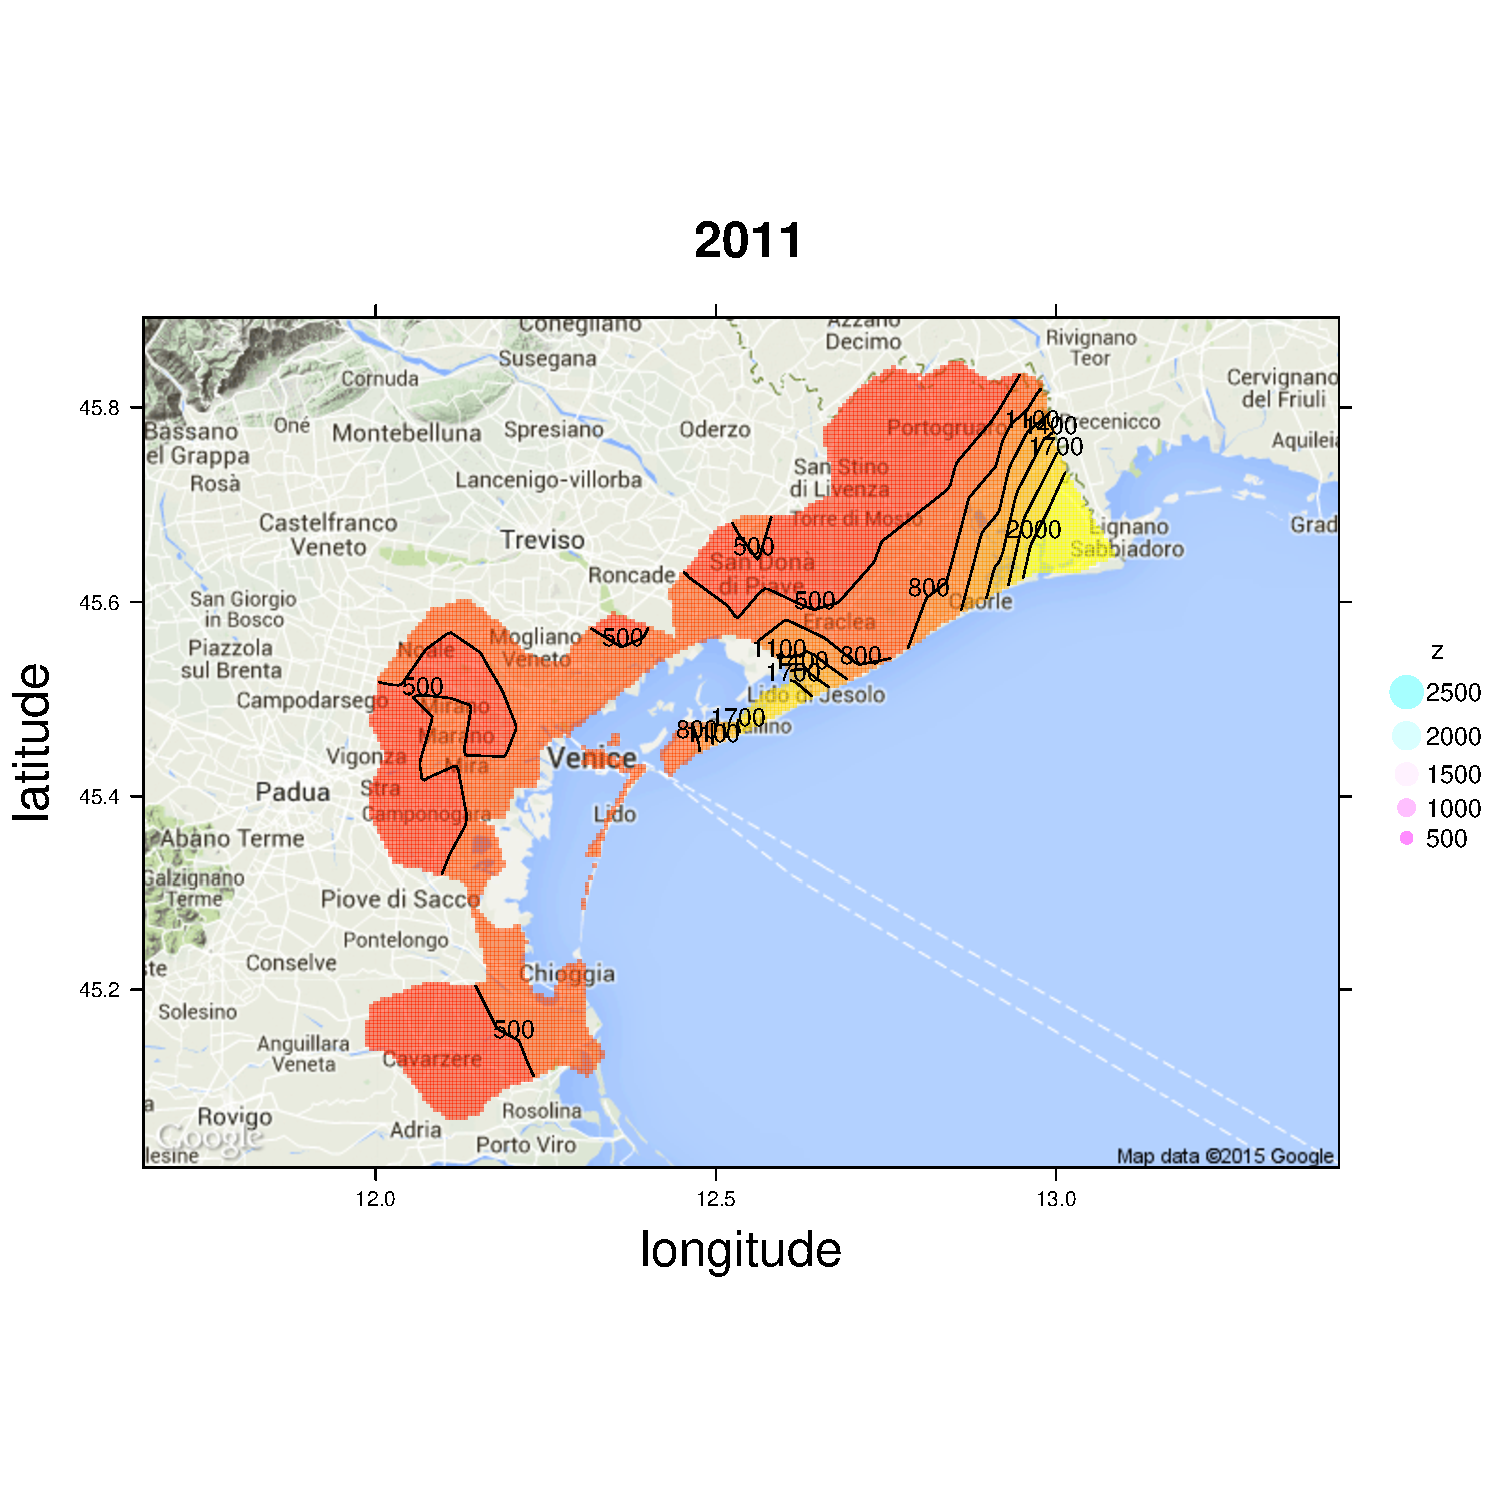
\includegraphics[trim=0cm 3cm 2.5cm 3.5cm,clip=true,width=0.8\textwidth]{immagini/Maps2011.pdf}
\caption{Estimated spatio-temporal field of the Venice waste data at a fixed time instant: year 2011.}
\label{fig:venezia_previsione}
\end{figure}
\begin{figure}[H]
\centering
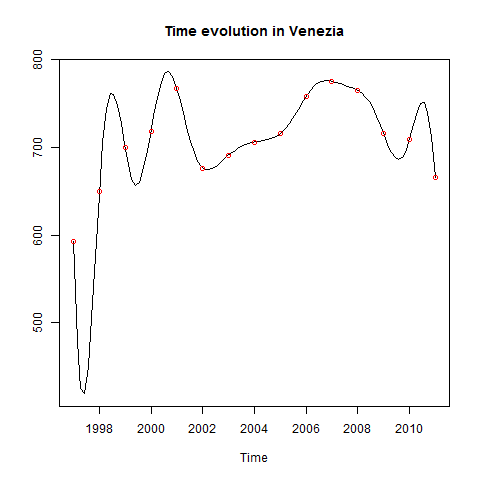
\includegraphics[width=0.32\textwidth]{immagini/Venezia.png}
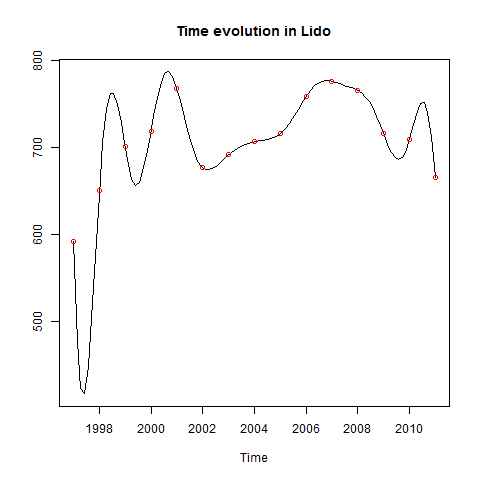
\includegraphics[width=0.32\textwidth]{immagini/Lido(A).png}
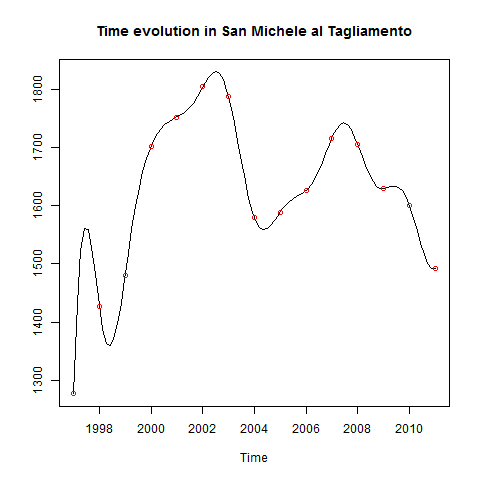
\includegraphics[width=0.32\textwidth]{immagini/SanMicheleTagliamento.png}
\caption{Estimated spatio-temporal field of the Venice waste data at three fixed spatial points: Venice, Lido and San Michele al Tagliamento.}
\label{fig:venezia_tempo}
\end{figure}


\subsubsection*{Comparison with other spatio-temporal prediction methods}

We compare our method with two other approaches to spatio-temporal fields estimation. The first method consists of a generalized additive mixed model with a tensor product of two smoothers in space and time; this algorithm is presented by Marra et al. in (\cite{art:marra}) and by Augustin et al. in (\cite{art:augustin}). The second method is spatio-temporal kriging with a separable variogram marginally exponential both in time and space, whose parameters are estimated from the empirical variogram.\\
We apply the three methods to simulated data on a C-shaped domain. We use the spatial test function $f$ that was used in (\cite{art:wood}) and we construct a spatio-temporal test function $g$ in the following way:
$$ g(\underline p,t)= f(\underline p) \cos(t) .$$



\begin{thebibliography}{9}

\bibitem{art:augustin}
Nicole H. Augustin, Verena M. Trenkel, Simon N. Wood, Pascal Lorance, \emph{Space-time modelling of blue ling for fisheries stock management}, Environmetrics, 24, 109–119, (2013)

\bibitem{art:marra}
Giampiero Marra, David L. Miller, Luca Zanin, \emph{Modelling the spatiotemporal distribution of the incidence of resident foreign population}, Statistica Neerlandica, 66, 133–160, (2012)

\bibitem{art:sangalli}
Laura M. Sangalli, James O. Ramsay, Timothy O. Ramsay, \emph{Spatial spline regression models}, Journal of the Royal Statistical Society: Series B, 75, 681–703, (2013)

\bibitem{art:wood}
Simon N. Wood, Mark W. Bravington, Sharon L. Hedley, \emph{Soap film smoothing}, Journal of the Royal Statistical Society: Series B, 70, 931–955, (2008)


%\bibitem{prog:R}
%R Core Team, \emph{R: A Language and Environment for Statistical Computing}, R Foundation for Statistical Computing, Vienna, 2013, \url{http://www.R-project.org/}

\end{thebibliography}

\end{document}



%\[ 
%\underset{\scriptscriptstyle (m\times 1)}{Y}= 
%\underset{\scriptscriptstyle (m\times n)}{X} 
%\underset{\scriptscriptstyle (n\times 1)}{B} 
%\]